%!TEX encoding = UTF-8 Unicode
%!TEX root = ../thesisCASes.tex

%% TITOLO
\section{Ecosistemi Udibili}
\label{sec:Ecosistemi Udibili}

Uno degli esiti musicali più importanti che ha portato con sé il paradigma della complessità è stato l'abbandono della scrittura come strumento unidirezionale di istruzione per l'ottenimento di suoni-conseguenze da strumenti, ed aver mosso la composizione verso la scrittura di interazioni e relazioni tra  strumenti.

%Uno degli esiti musicali più importanti che ha portato con sé 
%il paradigma della complessità, riguarda essenzialmente l'aver smesso di 
%scrivere musica per strumenti interattivi con cui farla (e viceversa), 
%ed esser passati invece al  comporre le interazioni tramite gli strumenti.

Da un punto di vista più generale, Heinz Von Foerster in tal senso 
sviluppò la teoria %dell'informazione
secondo cui l'informazione è un costrutto relazionale, 
e non solo un singolo oggetto o un solo segnale, 
e che di conseguenza la quantità di informazione in un sistema è determinata 
%quindi
dalla sua capacità di generare varietà.

Le implicazioni e le conseguenze di questo pensiero applicato alla musica sono enormi.
Nella nostra tradizione musicale occidentale, nell'insieme delle parole: Sistema Tonale, 
che sta a significare "quell'insieme delle regole di organizzazione ed uso dei
suoni maggiormente utilizzati per produrre musica" 
(sempre rimanendo nel contesto della tradizione musicale Occidentale), 
è frequente che passi in secondo piano la parola 
sistema, che assume invece un significato centrale nel contesto di questa tesi;
se si pensa che di conseguenza passa in secondo piano l'insieme di quelle relazioni
che compongono nella sua interezza un sistema, di cui parla Von Foerster, 
si riduce la pratica musicale ai minimi termini.

Non è un caso che molti compositori nel corso del XX Secolo, siano passati non solo al comporre 
i sistemi stessi con cui fare la propria musica, ma al comporne anche le interazioni.
Si pensi ai sistemi formalizzati come partiture da: Iannis Xenakis, John Cage, o Roland Kayn,
arrivando fino alle partiture comportamentali

\todo[inline,color=green]{luca fai attenzione, guaccero e chi come lui ha spinto la musica a quello che abbiamo ora, non avrebbe mai accettato che le sue partiture fossero definite comportamentali. Erano partiture, complete, dettagliate, più di altre, che permettono una musica più completa, più complessa di altre.}

come quelle di: Domenico Guaccero e 
del contesto generale della Roma del dopoguerra, per concludere con lavori di 
Karlheinz Stockhausen come Plus-Minus, dove i processi sono udibili.

%Tornando al tema principale, come accennato nell'abstract, 
Le interazioni che ho ritenuto importante affrontare 
all'interno dei sistemi creati dai compositori cibernetici sono di due tipi:
di sistemi che interagiscono con l’ambiente circostante appartenente al mondo fisico, 
e di sistemi che interagiscono con il proprio ambiente nel mondo digitale.
Prima di entrare nel merito del primo caso qui,
è doveroso spendere ancora qualche parola su cosa
si intenda per ambiente.

Nessun sistema è separabile e isolabile dall'ambiente circostante, 
a prescindere dal fatto che il suo spazio vitale, sia nel mondo fisico o digitale. 
Proprio come ha mostrato Heinz Von Foerster non si può parlare di auto-organizzazione
se non ci si riferisce essenzialmente a un ambiente che racchiuda il sistema al suo interno.
E nella pratica musicale, la sensibilità nel comporre le interazioni
è spesso lontana dall'idea del voler interagire con una consapevolezza effettiva del 
puntare ai cambiamenti di stato all'interno di un sistema con cui si interagisce;
a maggior ragione viene trascurata la possibilità di interagire con sistemi che abbiano
la capacità di auto-osservarsi non dipendendo più direttamente dal controllo dell'esecutore 
secondo delle modalità prettamente lineari, 
ma dall'ambiente, 
con la capacità di guardare al proprio stato interno per creare autonomamente le interazioni.
In particolare, nei sistemi auto-osservanti quello che si manifesta quando un sistema entra in interazioni non distruttive
con il proprio ambiente circostante, che coincide nella sostanza anche nel suo spazio vitale, è un Ecosistema.

\subsection{Audible EcoSystemics n.2 - Feedback Study}
\label{sec:Audible EcoSystemics n.2 - Feedback Study}

%In tal senso, 
I lavori del ciclo Ecosistemico Udibile di Agostino di Scipio, 
trovano fondamento a partire da fenomeni e relazioni che possono esistere e manifestarsi solamente nell'ambiente 
circostante da cui prende vita il sistema, 
che nel suo caso diventa proprio lo spazio acustico reale. 
Lavori come lo studio sul feedback, lo studio sul rumore di fondo, lo studio sulle risposte all'impulso, o
lo studio sul silenzio, sono nella loro essenza dei sistemi che hanno come principio 
nella loro morfogenesi, un determinato 
comportamento appartenente allo spazio acustico reale, delimitato in questi studi da una stanza
che ne racchiude al suo interno tutti gli agenti e le relazioni possibili,
per costruirne una storia di relazioni dove il sistema si osserva attraverso lo spazio fisico, 
(ambiente) e si manifesta e vive solo attraverso di esso.
In questo senso l’interprete, lo spazio, e gli ascoltatori, 
divengono essi stessi parte integrante del sistema, dove l’ascolto, diviene anche esso
parte dell’insieme delle cose e delle relazioni che lo costituisce. \\

\subsection{L'interazione Uomo-Macchina-Ambiente}
\label{sec:L'interazione Uomo-Macchina-Ambiente}

Qual'è dunque l'esigenza alla base del comporre le interazioni invece 
che limitarsi al comporre musica per strumenti interattivi? 
Superare la classica relazione uomo-macchina dominante nella tradizione musicale, 
iniziando a pensare invece allo sconfinato universo delle nuove possibilità della complessità.
Secondo Agostino Di Scipio, questo avviene in primo luogo grazie 
alla possibilità che la macchina possa rappresentarsi
senza mediazione umana, e attraverso l'ambiente circostante, \footcite{discipio_polverisonore_2016}
e dunque poi alla possibilità di stabilire un flusso di relazioni macchina-ambiente. 
Consentendo in secondo luogo al musicista e performer 
la possibilità di potersi aprire ad un flusso di relazioni 
complesso fra uomo-macchina-ambiente dove le tre sono fortamente connesse e interdipendenti 
l'una dall'altra.

\begin{figure}[h!]
\begin{center}
\vspace{0.5cm}
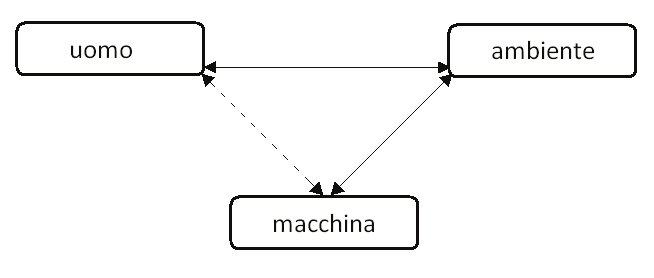
\includegraphics[width=8cm]{figures/uomo_macchina_ambiente.png} 
    \caption{Interazione Uomo-Macchina-Ambiente}
    \vspace{0.5cm}
\end{center}
\end{figure} 

\begin{quote}
la mossa decisiva è: passare da un lavoro che mira a usare mezzi interattivi per creare forme sonore desiderate ad
un lavoro che mira a creare le interazioni desiderate e ad ascoltarne le tracce udibili. Nel secondo caso, si tratta
di progettare, implementare, e rendere operativo un reticolo di componenti interconnesse il cui comportamento
sonoro emergente si può chiamare musica.\footcite{discipio_polverisonore_2016}
\end{quote}

La modalità con cui andrò a discutere in questo capitolo la composizione di interazioni ecosistemiche, 
è ponendo il focus su un lavoro di Agostino Di Scipio, l’Ecosistemico Udibile n.2, studio sul feedback. 
Partendo dalla partitura e dai suoi scritti, ed implementando e analizzando
il ruolo ed il compito dei singoli agenti all'interno del sistema 
che compongono nella loro totalità l'intero ecosistema del brano. 

\subsection{Il Meccanismo LAR}
\label{sec:Il Meccanismo LAR}

Il feedback elettroacustico, che abbiamo già detto
esser stata una delle risorse fondamentali dei primi compositori cibernetici,
è la condizione di partenza su cui Agostino Di Scipio opera per la costruzione dei suoi Ecosistemi Udibili.
Addentrandoci ora verso una spiegazione più tecnica del feedback elettroacustico,
possiamo citare una definizione che Di Scipio ha esposto in un suo articolo
pubblicato presso la rivista Online: ECHO dell’ Orpheus Institute, in
Ghent. \footcite{di_scipio_relational_2022}

\begin{quote}
A condenser microphone (M1) and a dynamic loudspeaker (L1) stand in the performance place
(S), few or several meters apart, maybe not too far from walls (or curtains, or other larger
surfaces). They are connected (through one or more amplification stages) to realize a very
basic electroacoustic chain: M1→L1→S. There’s no sound M1 should capture, though, no sound
source save the minimal, barely audible turbulence of the background noise, in a situation of
‘silence’. This ‘sound-of-nothing’ is amplified and heard through L1, whence it comes back in
S.

If amplification suffices, the L1 sound feeds back into M1 and the chain design closes onto
itself, making a ‘reinjection’ circuit – a feedback loop. The amplitude level, the
transductive technical features of M1 and L1, their relative distance, the distance from
walls, etc. – all of that (and much more) sets the actual feedback loop gain. With
not-too-high gain levels, what is engendered is an audible nuisance, a kind of ‘halo’: the
sound reinjection decays more or less rapidly, in a kind of badly sounding, spectrally uneven
reverb effect. With higher gain levels, the loop eventually enters a self-oscillatory regime,
it may ‘ring’ or ‘howl’, as is often said. Because of the iterated reinjection, the barely
audible but spectrally wide background noise accumulates in the loop and finally (quickly)
yields an increasingly louder sustained sound of narrower spectrum – this is often heard as a
peaking tone of definite pitch, or a tone cluster. That’s the Larsen effect: a self-sustaining
feedback resonance occasioned by a positive feedback loop (FB+) (‘positive’ here means greater
than unit gain).
\end{quote}

\begin{figure}[h!]
    \begin{center}
        \vspace{0.5cm}
        
\includegraphics[width=8cm]{figures/larsen_Feedback_scheme.png}
        \caption{Schema M1→L1→S}
        \vspace{0.5cm}
        \end{center}
\end{figure} 

L'effetto Larsen: (dal nome del fisico Søren Absalon Larsen
che per primo ne scoprì il principio), detto anche feedback elettroacustico,
come abbiamo appena letto è un fenomeno di retroiniezione che tende idealmente 
ad un'accumulazione infinita, che viene poi limitata in realtà dalla saturazione dei sistemi 
che la generano (relativi alla potenza massima, all'amplificazione, nonché alla sensibilità dei
trasduttori e all'elasticità delle membrane). Che può anche essere oltre al microfono, un
pick-up di uno strumento musicale elettrico, come una chitarra o un basso, o un trasduttore di
altra natura... 
Esistono anche principi di feedback acustico oltre che elettroacustico, 
come la risonanza acustica o la risonanza per simpatia,
che sono i principi su cui si basa il funzionamento di quasi tutti gli strumenti musicali. \\
Tornando quindi all'articolo di Agostino Di Scipio:

\begin{quote}
In common sound engineering practice, audible feedback phenomena are a nuisance, a problem one
should get rid of or substantially minimize. When direct level manipulation is not enough, one
resorts to hard-limiting circuits, ‘feedback killers’ and alike devices... 
In a different attitude, one may instead consider feedback as
a resource, a deliberately designed sound-making mechanism one can play with.\footcite{di_scipio_relational_2022}
\end{quote}

per utilizzare il feedback come una risorsa,
ora appare chiara la necessità di un intervento sulla sua retroiniezione a guadagno infinito 
che porta alla saturazione dei sistemi coinvolti, 
in tal senso una delle possibili soluzioni è quella di poter far calcolare
al computer in tempo reale tramite diverse tecniche di \textit{amplitude following} la stima dell'ampiezza
del segnale in ingresso, ed utilizzare conseguentemente la \textit{feature extraction} 
come segnale di controllo in retroazione negativa al sistema di feedback elettroacustico.

Questo tipo di meccanismi, provenienti dalla tradizione della Computer Music, appartiene 
all'ambito del \textit{Music Information Retrieval} (MIR).
Il MIR è un campo di ricerca multidisciplinare, che nell'area dell’informatica musicale si occupa di
studiare i metodi e gli strumenti per l’estrazione dell’informazione musicale per mezzo di un
computer.

Oltre alle analisi in tempo differito, che sono tipicamente trattate dal MIR
per le sue applicazioni di ricerca dove viene presa in considerazione
l’intera lunghezza del segnale su cui si effettua un analisi, 
oggi grazie ad alcuni linguaggi di programmazione
adatti alle implementazioni per il tempo reale e utili alle
performance in Live Electronics, è possibile operare anche alcune
di queste analisi in tempo reale, fra cui per l'appunto la stima dell'ampiezza
di un segnale in ingresso.
L'applicazione in tempo reale di una \textit{feature extraction} 
Nel contesto di una performance di live electronics, viene chiamata col nome di
\textit{Audio Information Processing};
tanto più un sistema è in grado di raccogliere informazioni riguardo
il suo stato e il suo rapporto con l'ambiente, tanto più sarà in grado di
processare "cognitivamente" tramite l'informazione il suo prodotto.

Rimandando al prossimo capitolo approfondimenti più dettagliati riguardo il tema 
dell'\textit{Audio Information Processing}, mi fermerò per il momento a discutere 
nel dettaglio alcuni fondamentali meccanismi presi da questo brano che sono paradigmatici,
come il singolo meccanismo di controbilanciamento del guadagno
del fenomeno di feedback elettroacustico, che viene chiamato da Agostino Di Scipio col nome di 
LAR: \textit{Audio feedback with self-regulated Gain},
e che può essere implementato in DSP in diverse modalità e configurazioni,
ognuna con le sue diverse caratteristiche e che porta a differenti esiti.

\begin{figure}[h!]
\begin{center}
\vspace{0.25cm}
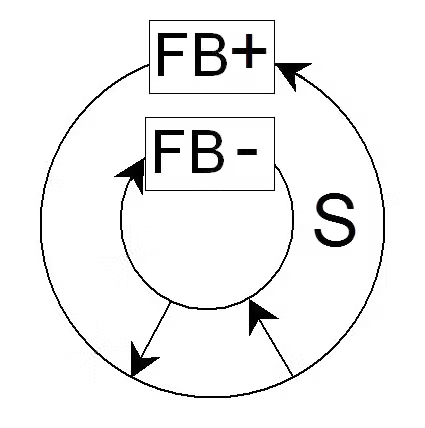
\includegraphics[width=4cm]{figures/controlled_larsen_Feedback.png}
\caption{Schema del meccanismo LAR}
\vspace{0.5cm}
\end{center}
\end{figure} 

Ci sono in effetti diversi modi per ottenere una \textit{feature extraction} 
in tempo reale capace di realizzare un algoritmo di controbilanciamento 
del feedback in tempo reale.
Alcuni di questi metodi possono riguardare controbilanciamenti 
applicati nel dominio della frequenza,
con tecniche di filtraggio automatizzate (adattive) che
hanno il compito di eliminare dallo spettro la presenza dell'autoscillazione prodotta dal Larsen \textit{Larsen Suppressors},
o come nel nostro caso d’interesse possono riguardare controbilanciamenti in ampiezza
automatizzati, che non permettano al feedback di avere un guadagno troppo troppo elevato 
e giungere conseguentemente allo stato di saturazione del sistema.
Algoritmi di \textit{amplitude-following} possono essere implementati 
con la media \textit{RMS}, con finestre variabili o fisse, 
filtri \textit{Peakholder} che mantengano il valore di picco, o di altra natura.

Tratterò a partire da ora nella tesi anche delle parti più operative, 
discutendo ed illustrando l'implementazione
di alcune di queste tecniche nel linguaggio di programmazione FAUST (Grame), 
che è uno dei linguaggi di programmazione
che consente di fare \textit{Audio Information Processing} in tempo reale.
Faust è l'ambiente in cui ho scritto i codici di tutti i lavori trattati
in questa tesi e le relative compilazioni, diagrammi e softwares.
\footnote{FAUST (Grame) (Functional Audio Stream), 
è un linguaggio di programmazione specifico per il Digital Signal
Processing sviluppato da Yann Orlarey, Dominique Fober, e Stephane Letz nel
2002. Nello specifico, FAUST è un linguaggio di programmazione ad alto livello
scritto in C++, che permette di tradurre delle istruzioni date e create 
appositamente per il digital signal processing (DSP), in un largo raggio di linguaggi
di programmazione non specifici per il dominio dell’Audio Digitale.} \footcite{https://faust.grame.fr/} \\
Vorrei qui esprimere la mia profonda gratitudine a 
Dario Sanfilippo per il prezioso supporto che mi ha fornito durante 
lo sviluppo di molti di questi codici,
e poiché nell'ultimo anno ha amorevolmente condiviso con me il suo sapere e le sue tecniche 
sviluppate nel corso dei suoi studi e delle sue ricerche, 
spiegandomi sempre con molta pazienza ogni dettaglio e applicazione 
di queste nei auoi sistemi complessi.

Il modo più semplice per mantenere l’effetto Larsen in uno stato stazionario, è attraverso un
valore costante ricavato dalla crescita del segnale in ingresso,
che controbilanci l’ampiezza del circuito di feedback come in figura del meccanismo LAR;
la stima di questa costante avviene tramite un algoritmo di analisi.
Il modo più semplice per implementare un algoritmo di analisi di questo tipo
è attraverso un \textit{Peakholder} che nella sua forma basilare consiste in una finestra 
di campioni idealmente infinita IIR \textit{Infinite Impulse Response},
e che può essere espresso matematicamente come

\begin{align*} 
    y_{1}(t) = \max\left( y_{1}(t\!-\!1), \left\lvert{x(t)}\right\rvert \right) 
\end{align*}

dove \textit{x} è il segnale in ingresso, e \textit{y} il segnale sia in uscita che reiterato nella funzione. \\
E utilizzato come algoritmo di controbilanciamento può essere espresso matematicamente come

\begin{align*} 
    y_{1}(t) = (1-(\max\left( y_{1}(t\!-\!1), \left\lvert{x(t)}\right\rvert \right))) * x(t)
\end{align*}

questo algoritmo ha il compito di confrontare il valore assoluto del campione in ingresso con il suo precedente,
e Il maggiore fra i due nella comparazione viene mandato sia in uscita che in ingresso 
in retroiniezione alla funzione stessa di comparazione, 
in questo modo si sfrutta un principio di feedback per l'accumulazione
del valore massimo, in un'analisi campione per campione.

\vspace{0.5cm} 
\lstinputlisting[breaklines, frame=trBL, caption={Algoritmo del \textit{Peakholder} ad 1 campione di ritardo}]
{codes/PeakholderIIR.dsp}

\vspace{0.5cm} 
\lstinputlisting[breaklines, frame=trBL, caption={Algoritmo del LAR con \textit{Peakholder} ad 1 campione di ritardo}]
{codes/LARpeakmax.dsp}

\begin{figure}[h!]
\begin{center}
    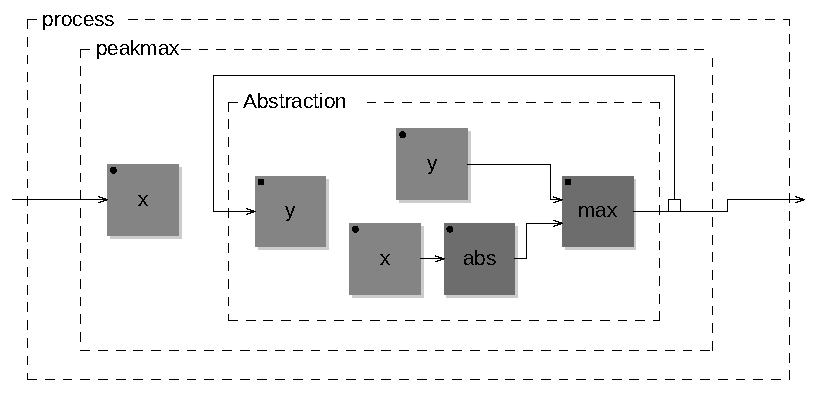
\includegraphics[width=14cm]{figures/PeakholderIIR.pdf}
    \caption{Topologia del \textit{Peakholder} ad 1 campione di ritardo} 
    \end{center}
\end{figure} 

\begin{figure}[h!]
\begin{center}
    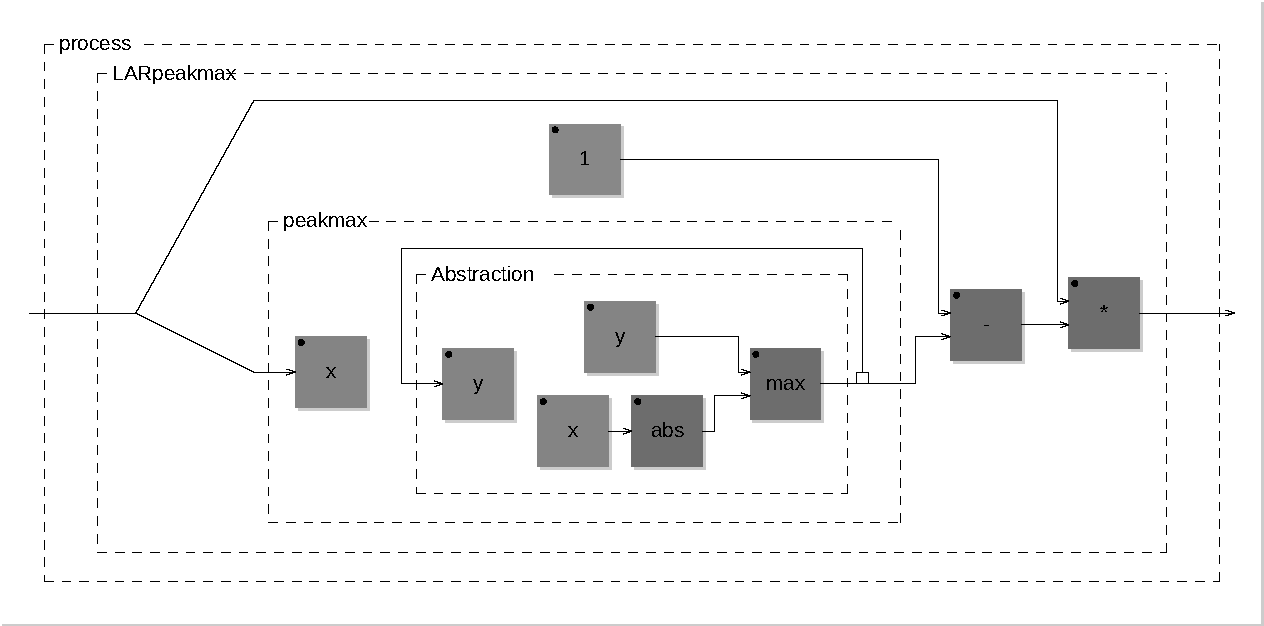
\includegraphics[width=14cm]{figures/LARpeakmax.pdf} 
    \caption{Topologia del LAR con \textit{Peakholder} ad 1 campione di ritardo} 
\end{center}
\vspace{0.5cm}
\end{figure} 

Questo tipo di algoritmo presenta comunque alcuni problemi: non avendo
una funzione di smoothing del segnale, si verificano problemi di segnali di differenza a banda
molto larga che possono generare aliasing e contributi spuri che tendono a permanere nel
segnale complessivo.
Oltre a questo, variazioni del comportamento del feedback sono dipendenti dalla grandezza
della finestra di osservazione, da eventuali cofficenti di feedback inseriti nella
retroazione del \textit{Peakholder} e da altri tipi di implementazioni di tecniche 
\textit{amplitude-following}. Per questi motivi si sceglie più frequentemente di utilizzare algoritmi
adattivi, proprio come nel contesto del meccanismo LAR implementato nel feedback study,
dove il comportamento adattivo dell'\textit{amplitude-follower} è cruciale
per la dinamica adattiva ed auto-regolatoria del sistema.

Il meccanismo LAR è essenzialmente nel cuore della live performance del feedback study,
senza di questo non sarebbe possibile creare una condizione favorevole per procedere alle 
conseguenti trasformazioni del suono, e conseguentemente ad una condizione favorevole affinché il 
sistema possa osservarsi tramite l'ambiente circostante. 
In tal senso vale la pena procedere osservando da vicino come viene richiesto in partitura 
di implementare questo meccanismo.

\begin{figure}[h!]
\begin{center}
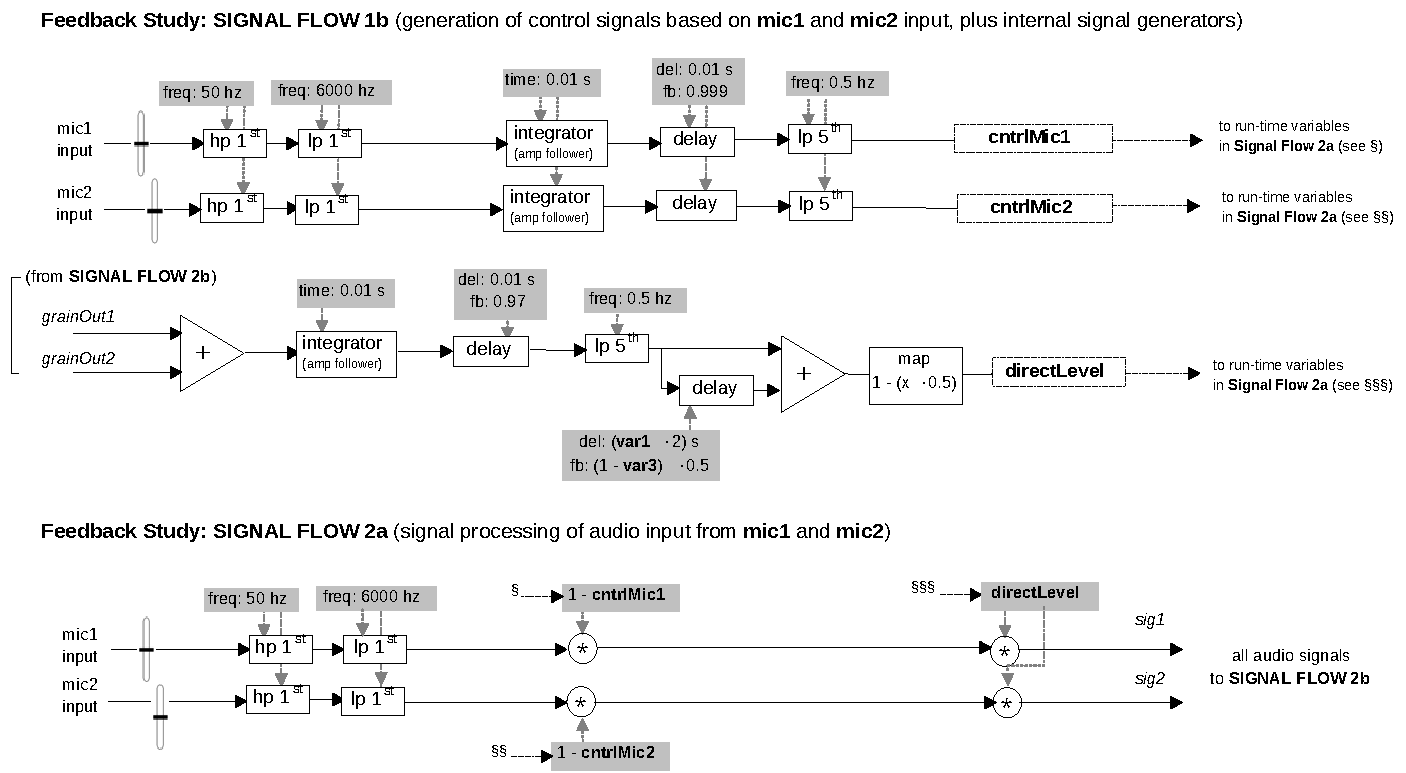
\includegraphics[width=14cm]{figures/LARFeedbackstudy2017.pdf}
\caption{Estratto dalla partitura di \textit{Audible Ecosystemics n.2/ feedback study (2003)}
revisione del 2017 - Agostino Di Scipio}
\vspace{0.5cm}
\end{center}
\end{figure}

Come scritto in partitura, è da notare in prima istanza
come il microfono serva sia da sorgente per l'alimentazione del Larsen che
da canale che riceve l'informazione necessaria per il meccanismo auto-regolatorio,
fin qui è tutto uguale rispetto allo Schema del meccanismo LAR.
La sostanziale differenza consiste invece nell'aggiunta di un secondo microfono,
quando viene introdotta questa condizione di disaccoppiamento si 
permette al meccanismo di essere più responsivo ai piccoli cambiamenti nell'ambiente
e di rispondere diversamente agli stessi stimoli da diversi punti di osservazione del sistema.

Nel \emph{Signal Flow 1b}, due microfoni in ingresso (\emph{mic1 e mic2}) 
vengono limitati in banda da un filtro \emph{highpass} ed 
un filtro \emph{lowpass}, rispettivamente fra $50Hz$ e $6000Hz$; dei due microfoni che escono 
dal \emph{cntrlMic1} e \emph{cntrlMic2} ne viene ricavato l'inviluppo d'ampiezza tramite
l'oggetto \emph{integrator}, poi la curva di questo inviluppo viene amplificata da 
un delay con feedback, e ne viene estratta solamente la componente energetica 
presente fra i $0Hz$ e i $0.5Hz$, limitandone il comportamento dell'oscillazione in quel range.
Più in basso, nel \emph{Signal Flow 2a}, i stessi microfoni (\emph{mic1 e mic2}) sempre
limitati in banda fra $50Hz$ e $6000Hz$, vengono attenuati in ampiezza dal segnale
proveniente dal \emph{cntrlMic1} e \emph{cntrlMic2}, realizzando nella sostanza una 
versione più sofisticata del contro-bilanciamento del meccanismo \emph{LAR}.
La parte restante: ovvero, la generazione del segnale \emph{directLevel} e la 
conseguente attenuazione dei segnali audio in uscita (\emph{sig1 e sig2}),
consiste in un secondo contro-bilanciamento ricavato da un processo di granulazione
attivo alla fine del sistema, finché il granulatore non produce segnale in output 
l'ampiezza dei segnali audio diretti in uscita dal sistema rimane inalterata.

L'inviluppo d'ampiezza ricavato tramite l'oggetto \textit{integrator}, in partitura 
viene richiesto come segue:

\begin{quote}
\begin{itemize}
  \item integrator = returns the average absolute value over a specific 
    time frame (one may use RMS measures, instead, or other amplitude-following methods); 
    output range is [0, 1]
\end{itemize}
\end{quote}

dove sostanzialmente, viene calcolato il valore assoluto di una specifica finestra temporale. 
A seguito una implementazione di questo tipo di algoritmo, dove \textit{fi.pole} è 
un semplice onepole filter nella forma

\begin{align*} 
    y(n) = x(n) + py(n-1)
\end{align*}

e \textit{ma.SR} una costante che rappresenta la frequenza di campionamento.

\vspace{0.5cm} 
\lstinputlisting[breaklines, frame=trBL, caption={Algoritmo d'integrazione a media mobile}]
{codes/MovingAverage.dsp}

In partitura viene indicato all'esecutore di poter utilizzare diversi metodi 
per poter calcolare il valore desiderato, come ad esempio l'RMS, 
tuttavia da analisi dirette secondo l'implementazione del compositore del sistema sul 
sistema hardware-software KYMA con il suo linguaggio di programmazione dedicato, 
i filtri utilizzati risultano essere di tipo IIR,
così da avere nella sostanza una risposta più lenta rispetto ad altre implementazioni come ad esempio 
quella del calcolo a media mobile.  
La risposta del filtro nell'implementazione originale è di tipo \textit{tau} 
e l'inviluppo è assoluto.

Se si desidera utilizzare questo tipo d'implementazione, nella libreria di Faust 
è possibile trovarla nell'oggetto \verb|an.abs_envelope_tau|.
Nella loro interezza i meccanismi di cntrlMic1 e cntrlMic2, e la conseguente
attenuazione del segnale diretto provenente da mic1 e mic2 
possono essere quindi implementati in Faust come segue:

\vspace{0.5cm} 
\lstinputlisting[breaklines, frame=trBL, caption={Algoritmo LAR nel feedback study}]
{codes/soloLAR_Audible_Ecosystemics_2.dsp}

Gli algoritmi degli oggetti richiamati in questa implementazione sono 
provenienti dalla libreria scritta per questo brano.
(sono stati riportati qui solo alcuni oggetti della libreria, per rendere eseguibile
il codice appena scritto)
Questo codice, che rappresenta il cuore del sistema,
permette grazie al meccanismo adattivo una condizione favorevole
per mantenere il Larsen in uno stato stazionario senza che giunga a 
saturazione, e consentendo al sistema
di fatto una serie di nuove possibilità di elaborazione e trasformazione del suono.

\subsection{Trasformazioni del suono}
\label{sec:Trasformazioni del suono}

l’Ecosistemico Udibile n.2, studio sul feedback, è costituito
da due principali meccanismi di feedback, uno nello spazio acustico reale,
e uno interno al sistema.

Il suono proveniente dal meccanismo LAR appena discusso nella precedente sezione,
passa per una serie di elaborazioni numeriche del segnale prima di essere restituito
e diffuso dagli altoparlanti nello spazio acustico reale. Queste elaborazioni
che vengono poi nuovamente intercettate dal microfono e riportate nel Sistema,
consentono una continua ed incessante trasformazione del suono, che permette
di cambiarne la morfologia ad ogni istante di tempo e in modo continuo, 
permettendo al sistema di avere "vita propria" ascoltandosi tramite l'ambiente
anche senza il contributo apportato da un esecutore.

Le elaborazioni del suono interne al sistema sono a loro volta di due tipologie,
\textit{sample read} e \textit{granular sampling}.

L'implementazione di questi due oggetti viene richiesta in partitura come segue:

\begin{quote}
\begin{itemize}
  \item sample write = write samples into a memory buffer, in cyclical fashion (wrap-around)
  \item sample read = read samples off the memory buffer, with controls over frequency shift ratios and actual buffer segment being read
  \item granular sampling = read sample sequences off subsequent buffer memory chunks, and envelopes the signal chunk with a pseudo-Gaussian envelope curve; the particular
    implementation should allow for time-stretching (slower memory pointer increments at grain level), as well as for "grain density" controls and slight random deviations ("jitter") on
    grain parameters; no frequency shift necessary
\end{itemize}
\end{quote}

dove \textit{sample write} rappresenta una tabella (buffer o dispositivo di memoria) 
che viene riscritta in modo continuo da un puntatore alla memoria;
ciclicamente, e in tutta la sua interezza.
La grandezza di questa tabella è data da una delle quattro variabili definite 
in partitura utilizzate per inizializzare il sistema, \textit{var1} che definito in questo contesto sta ad indicare
la grandezza della tabella in secondi.
Le 4 variabili definite per inizializzare il sistema ad ogni performance sono le seguenti:

\begin{quote}
\begin{itemize}
  \item var1 = distance (in meters) between the two farthest removed loudspeakers on the left-right axis.
  \item var2 = rough estimate of the center frequency in the spectrum of the room’s background noise (spectral centroid): to evaluate at rehearsal time, in a situation of "silence".
  \item var3 = subjective estimate of how the room revereberance, valued between 0 ("no reverb") and 1 (“very long reverb”).
  \item var4 = distance (in meters) between the two farthest removed loudspeakers on the front-rear axis.
\end{itemize}
\end{quote}

queste 4 variabili hanno un ruolo molto importante, poiché non solo vanno a determinare la velocità del
comportamento del sistema, ma ne vanno a determinare la sua sensibilità rispetto all'ambiente in cui viene 
eseguito, come ad esempio nel caso del \textit{sample read} la velocità di lettura dalla tabella \textit{sample write} 
e la porzione di tabella che ne viene letta.

I \textit{sample read} sono 5 indicati in partitura nella configurazione che segue.

\begin{figure}[h!]
\begin{center}
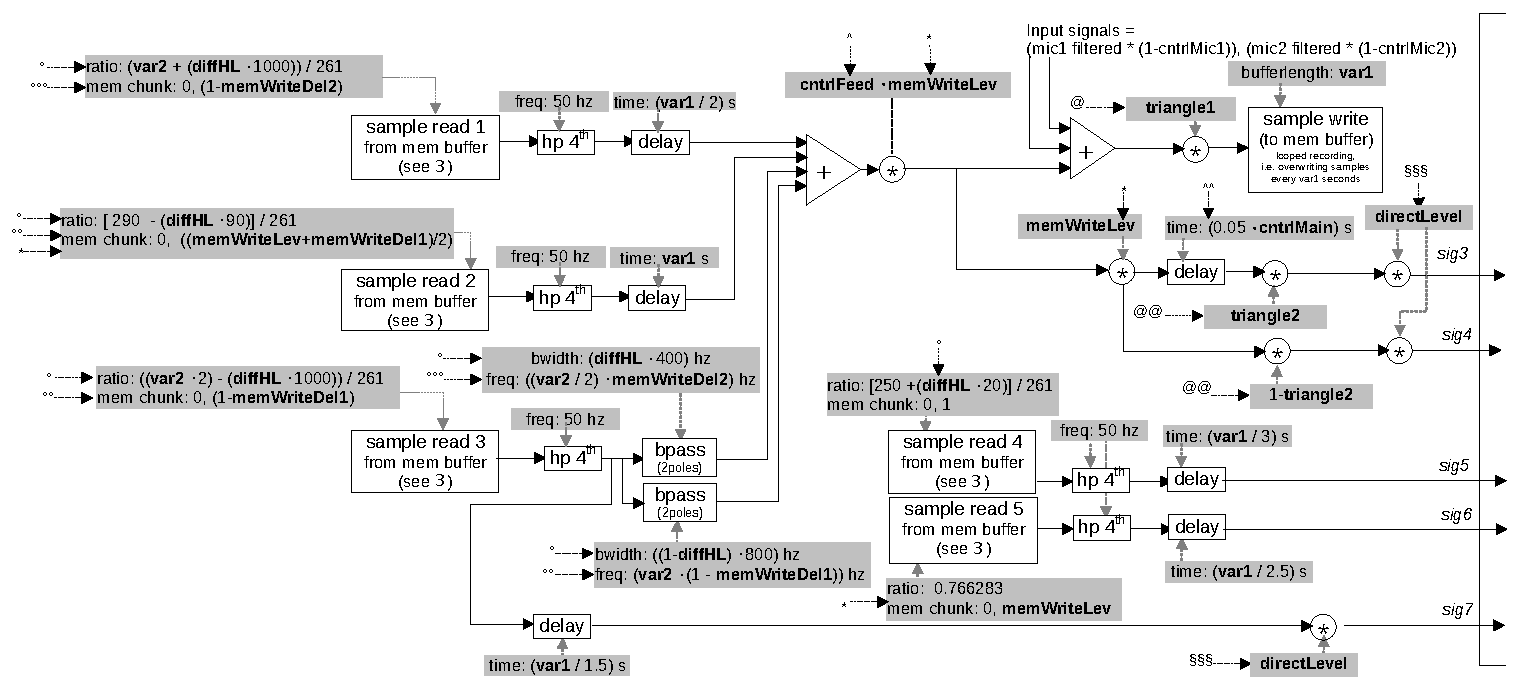
\includegraphics[width=14cm]{figures/SAMPLERSFeedbackstudy2017.pdf}
\caption{Estratto dalla partitura di \textit{Audible Ecosystemics n.2/ feedback study (2003)}
revisione del 2017 - Agostino Di Scipio} 
\vspace{0.5cm}
\end{center}
\end{figure} 

Il suono del Larsen proveniente da due microfoni e stabilizzato con il meccanismo LAR come 
illustrato in precedenza, viene a sommarsi per poi venire moltiplicato per un oscillatore a bassa frequenza
che ne modifica l'inviluppo d'ampiezza. Il risultato di questa operazione viene scritto in memoria
nella tabella \textit{sample write} e viene letto dai 5 campionatori distribuiti In
questa sezione del sistema.

I parametri esterni e tempo varianti che utilizza il campionatore sono: \textit{ratio} e \textit{mem chunk},
che corrispondono rispettivamente alla velocità di lettura e al frammento di buffer che viene letto
dalla tabella \textit{sample write}.
A seguito di una conversazione con il compositore è risultato essere fondamentale che
il campionatore aggiorni i valori di \textit{ratio} ad ogni campione, permettendo modulazioni
di frequenza derivate dal cambiamento delle velocità di lettura,
che si riflettono in cambiamenti di frequenza del Larsen registrato nel \textit{sample write}.
i \textit{ratio} vengono indicati in partitura con delle espressioni diverse per ognuno
dei 5 \textit{sample read}, ad esempio: \textit{ratio: (var2 + (diffHL * 1000)) / 261}, dove 

\begin{center}
    \vspace{0.5cm}
    \textit{ratio value sets the sample-read rate as a function of var2 and the control signal diffHL: ratio = 1 causes no rate
    change, hence no frequency shift of the sampled signal; values major of 1 determine shifts to higher frequencies; values
    between 0 and 1 determine shifts to lower frequencies}
    \vspace{0.5cm}
\end{center}

e dove \textit{diffHL} è un segnale
di controllo variabile in un range fra 0 e 1, che a run time a microfoni chiusi parte da una costante di 0.5.
La lettura del \textit{ratio} è sensibile rispetto all'ambiente, poiché il valore di \textit{diffHL}
che ne determina le modulazioni di frequenza, viene ricavato da una stima della centroide spettale 
nei segnali di controllo tramite una differenza fra filtri Highpass e Lowpass 
a cui viene passata come frequenza di taglio la variabile \textit{var2}.
Altrettanto sostanziale nel contribuire alle trasformazioni del Larsen 
è il comportamento del \textit{mem chunk}, che deve permettere una lettura
di frammenti di memoria che può andare dal silenzio: \textit{mem chunk: 0, 0} all'intera
lunghezza del buffer \textit{mem chunk: 0, 1}.
Anche in questo caso la maggiorparte dei campionatori implementa un \textit{mem chunk} 
determinato dai segnali di controllo variabili in un range fra 0 e 1, 
segnali di controllo che a run time e a microfoni chiusi 
partono da costanti distribuite di 0 e di 1.
Per questo motivo è molto importante che il comportamento del \textit{mem chunk} 
possa tollerare soglie ai due estremi.
In partitura altre importanti indicazioni sul campionatore che riguardano 
lettura e scrittura sono le seguenti:

\begin{center}
    \vspace{0.5cm}
    \textit{all sample-read processes 
    should include short fade-in and fade-out
    ramps when sampling pointers wrap around the buffer, to avoid
    discontinuities \\
    more discontinuities may occur because the buffer is being written
    as it is also being read: these can be avoided by various means of
    one's own design}
    \vspace{0.5cm}
\end{center}

In Faust non è possibile separare la scrittura e la lettura da un buffer,
difatti esistono solo 2 tipi di oggetti per questo scopo:
la primitiva \textit{rdtable}, che può essere utilizzata per leggere da una tabella di sola lettura 
(predefinita prima del tempo di compilazione),
e la primitiva \textit{rwtable}, che può essere utilizzata per implementare una tabella di lettura/scrittura. 
Quest'ultima prende in input un segnale che può essere scritto nella tabella utilizzando un indice di scrittura e 
letto utilizzando un secondo indice destinato alla lettura.
Per implementare in Faust l'architettura del \textit{sample write} richiesta in partitura, 
si possono sincronizzare gli indici di scrittura di tutte le tabelle con un unico 
segnale (rampa) destinato a questo scopo e utilizzato dai \textit{sample read} e dai \textit{granular sampling} 
impostando una grandezza comune, che risulta essere in questo caso una costante espressa in \textit{var1} in secondi, 
condivisa da tutti i buffer in questione.
In Faust la grandezza della tabella deve essere espressa in campioni. Per ottenere quindi
una grandezza espressa in secondi, bisogna dunque moltiplicare il numero dei secondi desiderati per
la frequenza di campionamento, definite entrambi come una costante (predefinita prima del tempo di compilazione).
Infine per completare le operazioni come richiesto nella partitura, si può sostituire l'oggetto \textit{rwtable}
con una mandata (send) del segnale destinato ad entrare in feedback ai \textit{sample read} ed in
feedforward al \textit{granular sampling}.
A seguito una implementazione del campionatore come richiesto in partitura.

\vspace{0.5cm} 
\lstinputlisting[breaklines, frame=trBL, caption={Algoritmo del \textit{sample write/read} per il feedback study}]
{codes/Sampler.dsp}

In questo campionatore, il \textit{ratio} è continuamente variabile, 
rendendo possibili le modulazioni di frequenza desiderate. 
Mentre il \textit{mem chunk} ricomincia la sua lettura del buffer dall'inizio 
ogni volta che la rampa di lettura incontra il valore del modulo determinato dalla sua variabile.
Per risolvere le discontinuità come richiesto in partitura, 
è necessario utilizzare un design personalizzato,
e nel design di questo campionatore, 
per evitare clicks ricorrenti ogni volta che la lettura del campionatore incrocia la sua scrittura, 
(visto che la lettura del \textit{mem chunk} parte sempre da inizio buffer)
la lettura parte solo quando la scrittura è di dimensioni maggiori rispetto al frammento \textit{mem chunk} 
che dovrebbe essere letto.
Infine, per evitare discontinuità ogni volta che la lettura ricomincia a leggere il buffer da 0, 
è stata utilizzata una finestratura trapezoidale con un fade-in e fade-out 
per un valore di campioni costante. \\
Mentre alcuni campionatori fanno parte di un circuito di feedback interno al sistema, 
sia i granulatori che tutti i campionatori utilizzano lo spazio acustico reale per il feedback,
i granulatori in particolare sono l'ultima trasformazione del suono del sistema, prima di andare a 
due sommatori con il resto delle uscite e all'output.
In partitura vengono indicati come a seguito.
\clearpage

\begin{figure}[h!]
\begin{center}
    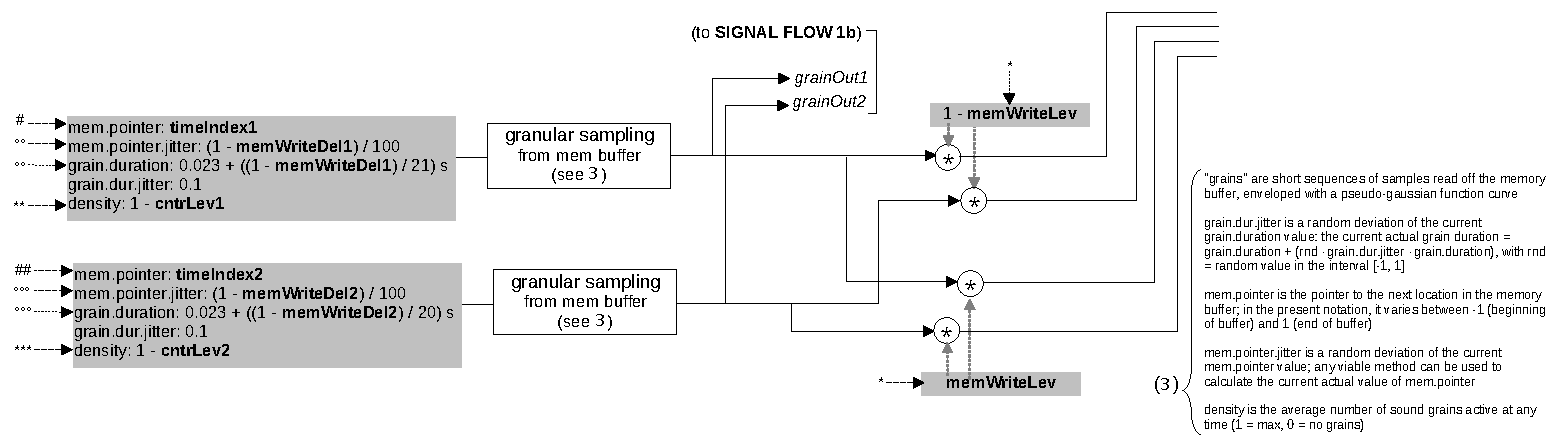
\includegraphics[width=14cm]{figures/GRANULATORSFeedbackstudy2017.pdf}
    \caption{Estratto dalla partitura di \textit{Audible Ecosystemics n.2/ feedback study (2003)}
    revisione del 2017 - Agostino Di Scipio}
    \vspace{0.5cm}
\end{center}
\end{figure}

Anche in questo caso, oltre alle indicazioni dei segnali di controllo che vengono
ricevuti dai due \textit{granular sampling}, 
in partitura sono presenti delle richiste specifiche riguardo l'implementazione 
dell'oggetto che ne determinano il risultato dei timbri che produce: 

\begin{center}
    \vspace{0.5cm}
    \textit{"grains" are short sequences of samples read off the memory
    buffer, enveloped with a pseudo-gaussian function curve \\
    grain.dur.jitter is a random deviation of the current
    grain.duration value: the current actual grain duration is:
    grain.duration + (rnd * grain.dur.jitter * grain.duration), with rnd
    is: random value in the interval (- 1, 1) \\
    mem.pointer is the pointer to the next location in the memory
    buffer; in the present notation, it varies between - 1 (beginning
    of buffer) and 1 (end of buffer) \\
    mem.pointer.jitter is a random deviation of the current
    mem.pointer value; any viable method can be used to
    calculate the current actual value of mem.pointer \\
    density is the average number of sound grains active at any
    time (1 is: max, 0 is: no grains)}
    \vspace{0.5cm}
\end{center}

I due granulatori leggono dunque dalla tabella \textit{sample write} dove vengono scritti
al contempo i Larsen diretti e i campionatori in feedback. 
Questa letura avviene con due puntatori alla memoria \textit{(mem.pointer)} determinati 
dai segnali di controllo \textit{timeIndex1} e \textit{timeIndex2}, la grandezza dei grani 
\textit{(grain.duration)} viene invece determinata dai segnali di controllo 
\textit{memWriteDel1} e \textit{memWriteDel2}, infine il parametro \textit{.jitter}
presente sia nei puntatori alla memoria che nelle durate (e calcolato in modo differente per ognuna delle due),
ha il compito di decorrelare le fasi dei grani, accedendo alla memoria in punti differenti,
e le durate di questi, dando vita in questo modo a delle tessiture timbriche \textit{"clouds"} più interessanti.
Anche in questo caso, a seguito di una conversazione con il compositore è emerso che le voci di polifonia
(istanze) risultano essere 10 per ogni \textit{granular sampling}.
Un problema che sorge nell'implementazione di un granulatore polifonico in un linguaggio di 
programmazione come Faust (che non contempla segnali di controllo ma lavora in DSP sul singolo campione),
è che in necessità di creare delle \textit{"clouds"}, è necessario che i puntatori di lettura
siano decorrelati in qualche modo, così da non non avere la stessa fase e sovrapporsi sistematicamente.
Nella tradizione della computer music, esistono diverse implementazioni techniche e design 
di algoritmi di granulazione per risolvere questo tipo di problema:
alcune tipologie di granulatori sono dette "asincrone" poiché sono particolari design dove
ogni istanza ha un personale \textit{trigger} 
di partenza che ne avvia la lettura del grano, decorrelato rispetto alle altre istanze,
invece e altre tipologie chiamate "quasi sincrone" e "sincrone" si concentrano sul mantenere
una coerenza di fase del segnale e una certa continuità.
In questo caso per il design di questo oggetto in Faust, si è optato per un tipo di granulazione
PSOLA (acronimo di Pitch-Synchronous Overlap and Add, sovrapposizione e aggiunta a toni sincroni), 
poiché come abbiamo visto precedentemente in partitura, 
seppur sono presenti funzioni di \textit{jittering} del segnale
per ottenere certe tessiture timbriche, viene esplicitamente richiesto
che il \textit{timestretching} del suono sia possibile. 
A seguito una implementazione del granulatore come richiesto in partitura.

\vspace{0.5cm} 
\lstinputlisting[breaklines, frame=trBL, caption={Algoritmo del \textit{granular sampling} per il feedback study}]
{codes/Granulator.dsp}

\subsection{Conclusioni}
\label{sec:Conclusioni}

In conclusione, abbiamo avuto modo di approfondire alcuni dei principali meccanismi 
utilizzati da Agostino Di Scipio per uno dei più importanti lavori del suo ciclo Ecosistemico Udibile,
prendendo questo lavoro come caso di studio con il fine di illustrare alcune modalità e relazioni possibili 
di un sistema con l'ambiente circostante e lo spazio acustico.
I meccanismi contenuti all'interno del brano ovviamente non si limitano a questi,
e ci sono altre modalità d'interazione con l'ambiente circostante prodotte da altri meccanismi di elaborazione
digitale del suono; così come ne esistono delle altre tipologie in altri lavori del ciclo tanto quanto 
nell'operato di altri compositori, ma si è cercato qui di illustrare alcuni passaggi 
essenziali così da poter lasciar spazio ad ulteriori approfondimenti dedicati ad altri sistemi di 
altro tipo, lasciando comunque aperta la possibilità di poter approfondire il brano a partire
dai testi citati in bibliografia e dal codice di un porting dell'intero sistema in Faust 
riportato nell'appendice.